%%% ===============================================================================
%                                  CHAPTER 2
%%% ===============================================================================
% Proposed preamble additions: none. The chapter uses only packages and macros that the
% preamble already provides (siunitx, booktabs, tikz via pgfplots, zref-clever, \todo).
\chapter{Background and Related Work}\label{ch:background}

This chapter provides the background that the method of \zcref{ch:method} and the results of the later chapters rely on, and it places the thesis in the literature on the energy of machine learning.
\Zcref{sec:rl-prelim} introduces the concepts of reinforcement learning that the four algorithms share, and \zcref{sec:algos} describes the algorithms as published and introduces the segments of a training loop to which the thesis attributes energy.
\Zcref{sec:energy-measurement} explains how energy is read from commodity hardware and what the tools that do so measure, and \zcref{sec:compute-accounting} defines the counting convention for floating-point operations and the energy per FLOP.
\Zcref{sec:related} reviews related work on the energy of machine learning, on the accuracy of software energy meters, on the estimation of energy from FLOPs and on compute and energy in reinforcement learning, and it ends with the knowledge gap that the research questions of \zcref{ch:method} address.
Only concepts that a later chapter uses are introduced; the implementations used in the experiments, and where they deviate from the publications, are described in \zcref{sec:alg-segments} and \zcref{sec:baselines}.


%%% ===============================================================================
%                                  SECTION 2.1
%%% ===============================================================================
\section{Reinforcement Learning Preliminaries}\label{sec:rl-prelim}

This section introduces the concepts of reinforcement learning (RL) that the four algorithms of \zcref{sec:algos} build on.
It follows the textbook of Sutton and Barto~\cite{sutton2018rl} and defines only what the later chapters use.

\paragraph{Markov decision process and objective.} An RL agent interacts with an environment in discrete time steps.
At step $t$, it observes a state $s_t$, chooses an action $a_t$ according to its \emph{policy} $\pi(a \mid s)$, receives a scalar reward $r_t$ and observes the next state $s_{t+1}$.
This setting is formalised as a \emph{Markov decision process} (MDP) with states $\mathcal{S}$, actions $\mathcal{A}$, a transition distribution $p(s' \mid s, a)$, a reward function $r(s,a)$ and a discount factor $\gamma \in [0,1)$.
In the two tasks of this thesis, the state is a vector of joint positions and velocities, and the action is a vector of bounded joint torques, so that the action dimension $|\mathcal{A}|$ is the number of actuated joints.
The agent aims to maximise the expected discounted return
\begin{equation}
  J(\pi) = \mathbb{E}_{\pi}\Bigl[\sum_{t=0}^{\infty} \gamma^{t} r_t\Bigr] .
  \label{eq:bg-return}
\end{equation}

\paragraph{Termination and time limit.} An episode ends either when the environment reaches a terminal state (\emph{termination}) or when a time limit is reached (\emph{truncation})~\cite{towers2024gymnasium}.
The two cases are treated differently when values are estimated: after a termination no further reward can be collected, whereas after a truncation the episode would have continued, so the value of the last state is still bootstrapped.
Let $\eta \in \{0,1\}$ denote the terminal flag of a transition.
An algorithm that imagines trajectories with a learned model must also predict termination if the task has terminal states.

\paragraph{Value functions and the Bellman equation.} The action-value function $Q^{\pi}(s,a)$ is the expected return when the agent takes action $a$ in state $s$ and follows $\pi$ afterwards.
It satisfies the Bellman equation
\begin{equation}
  Q^{\pi}(s,a) = \mathbb{E}\Bigl[r_t + \gamma\,(1-\eta_{t+1})\,Q^{\pi}(s_{t+1},a_{t+1}) \,\Bigm|\, s_t = s,\ a_t = a\Bigr] .
  \label{eq:bg-bellman}
\end{equation}
The next action $a_{t+1}$ is drawn from $\pi(\cdot \mid s_{t+1})$.
Learning methods turn this equation into a regression problem.
A function approximator $Q_{\phi}$ with parameters $\phi$, the \emph{critic}, is trained on transitions $(s,a,r,s',\eta)$ towards the \emph{target}
\begin{equation}
  y = r + \gamma\,(1-\eta)\,V_{\mathrm{next}}(s'),
  \label{eq:bg-td-target}
\end{equation}
where $V_{\mathrm{next}}(s')$ is an estimate of the value of the next state that each algorithm defines in its own way (\zcref{sec:algos}).
The critic minimises the squared difference between $Q_{\phi}(s,a)$ and $y$ averaged over a minibatch, which is called temporal-difference learning.

\paragraph{Off-policy learning and the replay buffer.} An algorithm is \emph{off-policy} if it can learn from transitions that were generated by an older version of the policy or by a different policy.
All four algorithms of this thesis store their transitions in a \emph{replay buffer}~\cite{lin1992replay} and train on minibatches of $B$ transitions drawn from it.
Reusing stored data makes learning more sample-efficient than discarding it after one update, and it decouples the number of gradient steps from the number of environment steps.
The policy that selects actions during data collection is the \emph{behaviour policy}; it usually contains exploration noise.
Before learning starts, the buffer is filled with transitions from random actions (the \emph{warmup}).

\paragraph{Actor-critic methods.} In an actor-critic method, a second approximator, the \emph{actor} $\pi_{\theta}$, is improved with the help of the critic.
For a deterministic actor, the update follows the gradient of the critic with respect to the action, $\nabla_a Q(s,a)\,\nabla_{\theta}\pi_{\theta}(s)$, which is the deterministic policy gradient~\cite{silver2014dpg,lillicrap2016ddpg}.
For a stochastic actor, the gradient is propagated through a sampled action that is written as a differentiable function of the parameters and of independent noise.
Both variants alternate between a critic update and an actor update.

\paragraph{Target networks and Polyak averaging.} The target in \zcref{eq:bg-td-target} depends on the critic that is being trained, which can make learning unstable.
\emph{Target networks} address this: a second copy $\bar{\phi}$ of the critic, which changes slowly, is used to compute $V_{\mathrm{next}}$~\cite{mnih2015dqn}.
In continuous control, the copy is usually updated after every gradient step by \emph{Polyak averaging}~\cite{polyak1992averaging,lillicrap2016ddpg},
\begin{equation}
  \bar{\phi} \leftarrow (1-\tau)\,\bar{\phi} + \tau\,\phi,
  \label{eq:bg-polyak}
\end{equation}
where $\tau \ll 1$ is the \emph{Polyak coefficient}.
The update is a weighted sum of two parameter vectors and contains no matrix product, which matters for how it is counted in \zcref{sec:compute-accounting}.

\paragraph{Update-to-data ratio.} The \emph{update-to-data ratio} $U$ is the number of gradient updates per environment step, also called the replay ratio~\cite{fedus2020replay}.
A run with $N_{\mathrm{env}}$ environment steps performs $N_{\mathrm{env}}\,U$ updates.
Standard actor-critic algorithms use $U = 1$.
Methods that gain sample efficiency from a larger ratio include REDQ~\cite{chen2021redq}, MBPO~\cite{janner2019mbpo} and resetting-based agents~\cite{doro2023replayratio}.
A change of $U$ changes how often an update is executed, not what one update costs: the cost per update is set by the networks and the batch size.
\Zcref{sec:flop-counts} uses this to reconstruct the number of calls of each segment.

\paragraph{Model-based reinforcement learning.} A \emph{model-based} algorithm learns a model $\hat{p}(s', r \mid s, a)$ of the environment from the collected data and uses it in addition to, or instead of, further interaction.
The Dyna idea~\cite{sutton1991dyna} uses the model to generate additional, synthetic transitions for a learner that would otherwise only see real ones.
Because the error of a learned model compounds along a trajectory, MBPO~\cite{janner2019mbpo} starts short model rollouts from states that were observed in the real environment and stores the generated transitions in a separate \emph{model buffer}; such rollouts are called \emph{branched}.
To represent uncertainty about the dynamics, the model is an \emph{ensemble} of probabilistic networks that each predict a distribution over the next state~\cite{chua2018pets}.

\paragraph{Latent world models and MPPI.} A \emph{latent world model} does not predict raw observations.
It learns an encoder $z = h_{\theta}(s)$ that maps the observation to a compact latent state and a dynamics function $z' = f_{\theta}(z,a)$ that advances this state, together with heads that predict the reward $\hat{r}_{\theta}(z,a)$ and a value $Q_{\theta}(z,a)$, and a policy $p_{\theta}(z)$ that maps a latent state to an action~\cite{hansen2022tdmpc}.
Actions are then not read from a policy alone but found by planning inside the model.
\emph{Model predictive path integral} control (MPPI)~\cite{williams2017mppi} does this by sampling.
It keeps a Gaussian distribution over action sequences of length $H$ (the \emph{horizon}).
In each of several \emph{iterations}, it draws a number of \emph{samples} from this distribution, evaluates each sequence in the model, advancing the latent state by $z_{t+1} = f_{\theta}(z_t,a_t)$ from $z_0 = h_{\theta}(s_t)$, by the predicted return
\begin{equation}
  G(a_{0:H-1}) = \sum_{t=0}^{H-1} \gamma^{t}\,\hat{r}_{\theta}(z_t,a_t) + \gamma^{H}\,Q_{\theta}\bigl(z_H, p_{\theta}(z_H)\bigr),
  \label{eq:bg-mppi-score}
\end{equation}
keeps the best \emph{elites}, and refits the mean and the standard deviation of the distribution to them with weights that increase with the return.
Some of the samples can be \emph{seeded} from the learned policy $p_{\theta}$, which is then called the policy prior.
After the last iteration, the first action of the resulting sequence is executed in the environment, and the planning is repeated at the next step.


%%% ===============================================================================
%                                  SECTION 2.2
%%% ===============================================================================
\section{The Four Algorithms}\label{sec:algos}

The thesis studies four algorithms from three families: the model-free actor-critic methods SAC and TD3, the model-based method MBPO, and the planning-based method TD-MPC2.
This section describes each algorithm as published and names the parts of its training loop that the later chapters treat as \emph{segments}.
A segment is a phase of the loop to which the thesis attributes energy; the vocabulary is shared by all four algorithms:
\begin{itemize}
  \item \emph{rollout}: interaction with the environment, including the choice of the action;
  \item \emph{buffer sample}: drawing a minibatch from the replay buffer;
  \item \emph{critic update}: one gradient step on the critic;
  \item \emph{actor update}: one gradient step on the actor;
  \item \emph{target update}: the Polyak averaging of the target networks;
\end{itemize}
and the segments that exist for one algorithm only: the \emph{model fit} and the \emph{synthetic rollouts} of MBPO, and the \emph{planning} and the \emph{world-model pretraining} of TD-MPC2.
The first five are the segments of SAC, which defines the reference structure.
\Zcref{tab:alg-iteration} summarises what one iteration of each algorithm contains, and \zcref{fig:alg-loops} shows the order of the segments.
The way in which the instrumented implementations measure these segments, and what the shared names mean for each algorithm, is the subject of \zcref{sec:measured-allocated}, \zcref{tab:status} and \zcref{tab:segment-meaning}.

\begin{table}[tbp]
  \centering
  \footnotesize
  \caption{What an iteration of each algorithm contains, as published.
    $Q_1, Q_2$ are the twin critics, $\bar{Q}$ denotes target critics, and $d$ is the policy-update delay (\zcref{sec:algo-td3}).}
  \label{tab:alg-iteration}
  \begin{tabular}{@{}p{2.3cm}p{2.5cm}p{2.5cm}p{2.5cm}p{3.0cm}@{}}
    \toprule
    Aspect              & SAC                                    & TD3                                          & MBPO                                  & TD-MPC2                                          \\
    \midrule
    Acting              & sample from the stochastic policy      & deterministic action plus Gaussian noise     & as SAC                                & MPPI planning in latent space                    \\
    Learned components  & policy, $Q_1, Q_2$, temperature        & policy, $Q_1, Q_2$                           & SAC components and dynamics ensemble  & encoder, latent dynamics, reward head, Q-ensemble, policy prior \\
    Critic target       & $\min \bar{Q}_i$ minus entropy term    & $\min \bar{Q}_i$ at a smoothed target action & as SAC                               & reward plus $\min$ of two random target Qs       \\
    Actor objective     & value minus entropy term               & gradient of $Q_1$                            & as SAC                                & value with entropy bonus, on latents             \\
    Actor and targets   & every update                           & every $d$-th update                          & every update                          & every update                                     \\
    Training data       & replay buffer                          & replay buffer                                & model buffer (synthetic transitions)  & sequences of consecutive steps from the buffer   \\
    Further stages      & --                                     & --                                           & model fit, synthetic rollouts         & pretraining on seed data                         \\
    \bottomrule
  \end{tabular}
\end{table}

\begin{figure}[tbp]
  \centering
  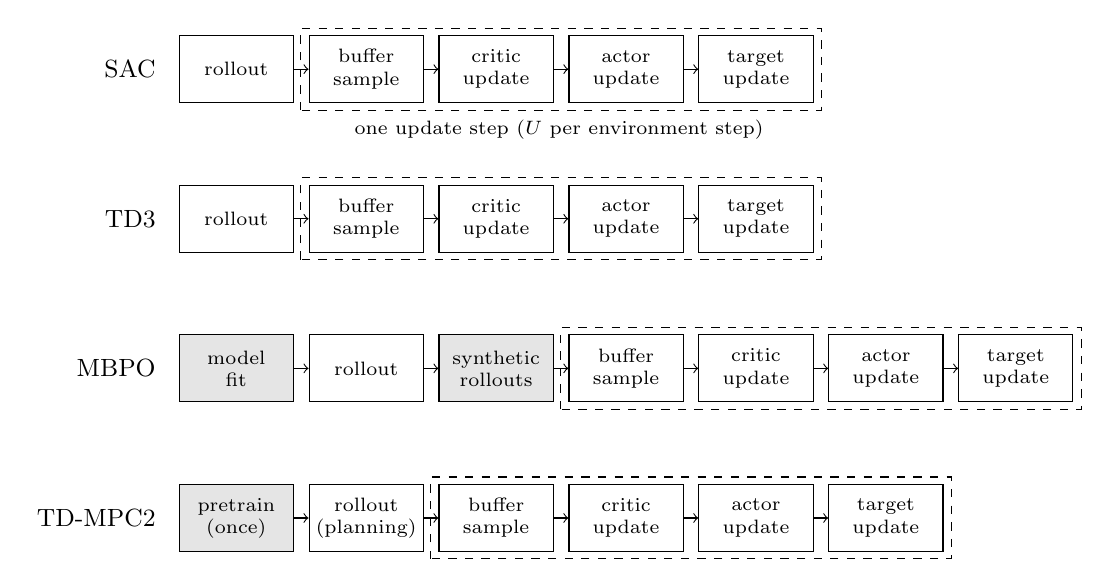
\begin{tikzpicture}[font=\scriptsize,
      seg/.style={draw, minimum width=1.45cm, minimum height=0.85cm, align=center, inner sep=1pt},
      ext/.style={seg, fill=black!10}]
    % SAC
    \node[anchor=east,font=\small] at (1.1,0) {SAC};
    \node[seg] (a0) at (2.0,0) {rollout};
    \node[seg] (a1) at (3.65,0) {buffer\\sample};
    \node[seg] (a2) at (5.3,0) {critic\\update};
    \node[seg] (a3) at (6.95,0) {actor\\update};
    \node[seg] (a4) at (8.6,0) {target\\update};
    \draw[->] (a0) -- (a1); \draw[->] (a1) -- (a2); \draw[->] (a2) -- (a3); \draw[->] (a3) -- (a4);
    \draw[dashed] (2.82,-0.52) rectangle (9.43,0.52);
    \node[anchor=north] at (6.1,-0.52) {one update step ($U$ per environment step)};
    % TD3
    \node[anchor=east,font=\small] at (1.1,-1.9) {TD3};
    \node[seg] (b0) at (2.0,-1.9) {rollout};
    \node[seg] (b1) at (3.65,-1.9) {buffer\\sample};
    \node[seg] (b2) at (5.3,-1.9) {critic\\update};
    \node[seg] (b3) at (6.95,-1.9) {actor\\update};
    \node[seg] (b4) at (8.6,-1.9) {target\\update};
    \draw[->] (b0) -- (b1); \draw[->] (b1) -- (b2); \draw[->] (b2) -- (b3); \draw[->] (b3) -- (b4);
    \draw[dashed] (2.82,-2.42) rectangle (9.43,-1.38);
    % MBPO
    \node[anchor=east,font=\small] at (1.1,-3.8) {MBPO};
    \node[ext] (c0) at (2.0,-3.8) {model\\fit};
    \node[seg] (c1) at (3.65,-3.8) {rollout};
    \node[ext] (c2) at (5.3,-3.8) {synthetic\\rollouts};
    \node[seg] (c3) at (6.95,-3.8) {buffer\\sample};
    \node[seg] (c4) at (8.6,-3.8) {critic\\update};
    \node[seg] (c5) at (10.25,-3.8) {actor\\update};
    \node[seg] (c6) at (11.9,-3.8) {target\\update};
    \draw[->] (c0) -- (c1); \draw[->] (c1) -- (c2); \draw[->] (c2) -- (c3); \draw[->] (c3) -- (c4); \draw[->] (c4) -- (c5); \draw[->] (c5) -- (c6);
    \draw[dashed] (6.12,-4.32) rectangle (12.73,-3.28);
    % TD-MPC2
    \node[anchor=east,font=\small] at (1.1,-5.7) {TD-MPC2};
    \node[ext] (d0) at (2.0,-5.7) {pretrain\\(once)};
    \node[seg] (d1) at (3.65,-5.7) {rollout\\(planning)};
    \node[seg] (d2) at (5.3,-5.7) {buffer\\sample};
    \node[seg] (d3) at (6.95,-5.7) {critic\\update};
    \node[seg] (d4) at (8.6,-5.7) {actor\\update};
    \node[seg] (d5) at (10.25,-5.7) {target\\update};
    \draw[->] (d0) -- (d1); \draw[->] (d1) -- (d2); \draw[->] (d2) -- (d3); \draw[->] (d3) -- (d4); \draw[->] (d4) -- (d5);
    \draw[dashed] (4.47,-6.22) rectangle (11.08,-5.18);
  \end{tikzpicture}
  \caption{Order of the segments in the training loops, as published.
    Shaded boxes exist for one algorithm only.
    The dashed frame is one update step, which is repeated $U$ times per environment step.
    In TD3, the actor and target updates run only on every $d$-th update.
    For TD-MPC2, the pretraining runs once before the loop, and for MBPO the model fit and the synthetic rollouts run once per block of environment steps.
    In the instrumented implementations the order differs (\zcref{sec:epoch-tasks}).}
  \label{fig:alg-loops}
\end{figure}

\subsection{Soft Actor-Critic}\label{sec:algo-sac}

Soft Actor-Critic (SAC)~\cite{haarnoja2018sac} is an off-policy actor-critic method with a stochastic actor.
It maximises the return of \zcref{eq:bg-return} plus an entropy bonus that rewards randomness of the policy, weighted by a \emph{temperature} $\alpha$.
The entropy term keeps the policy exploring and makes the learned behaviour robust.
The form used in the experiments is the later version of the algorithm~\cite{haarnoja2018sacapps}, in which the temperature is tuned automatically.

SAC learns two critics $Q_{\phi_1}, Q_{\phi_2}$ (\emph{twin critics}) with target copies $Q_{\bar{\phi}_1}, Q_{\bar{\phi}_2}$.
Both are trained towards the same target, which uses the smaller of the two target values,
\begin{equation}
  y = r + \gamma\,(1-\eta)\Bigl(\min_{i \in \{1,2\}} Q_{\bar{\phi}_i}(s',a') - \alpha \log \pi_{\theta}(a' \mid s')\Bigr),
  \label{eq:bg-sac-target}
\end{equation}
where the next action $a'$ is sampled from the current policy $\pi_{\theta}(\cdot \mid s')$.
Taking the minimum counteracts the overestimation of values that a single maximising critic suffers from.
The idea goes back to double Q-learning~\cite{vanhasselt2010doubleq} and is called \emph{clipped double Q-learning} in the form used by TD3 (\zcref{sec:algo-td3}).
The actor is a Gaussian whose sample is squashed into the valid action range, and it is updated to minimise
\begin{equation}
  L_{\pi}(\theta) = \mathbb{E}_{s \sim \mathcal{D},\, a \sim \pi_{\theta}}\bigl[\alpha \log \pi_{\theta}(a \mid s) - \min_{i} Q_{\phi_i}(s,a)\bigr],
  \label{eq:bg-sac-policy}
\end{equation}
that is, to prefer actions with a high value and a high entropy.
The temperature is adapted by a gradient step on
\begin{equation}
  L_{\alpha} = \mathbb{E}_{s \sim \mathcal{D},\, a \sim \pi_{\theta}}\bigl[-\alpha\,(\log \pi_{\theta}(a \mid s) + \bar{\mathcal{H}})\bigr],
  \label{eq:bg-sac-temp}
\end{equation}
so that the entropy of the policy approaches a \emph{target entropy} $\bar{\mathcal{H}}$.
The published setting is $\bar{\mathcal{H}} = -|\mathcal{A}|$, the negative action dimension~\cite{haarnoja2018sacapps}.
After each update, the target critics follow the critics by Polyak averaging (\zcref{eq:bg-polyak}).

In terms of segments, an iteration of SAC consists of a \emph{rollout} step in which an action is sampled from the policy and stored, and an update step with the \emph{buffer sample}, the \emph{critic update}, the \emph{actor update} (policy and temperature) and the \emph{target update} of the two critics.
SAC is the reference algorithm of the thesis because its structure is the simplest and is contained in the other three.

\subsection{Twin Delayed Deep Deterministic Policy Gradient}\label{sec:algo-td3}

TD3~\cite{fujimoto2018td3} extends the deterministic actor-critic algorithm DDPG~\cite{lillicrap2016ddpg}, which in turn builds on the deterministic policy gradient~\cite{silver2014dpg}, by three changes that reduce the overestimation of values.
First, it uses \emph{clipped double Q-learning}: two critics are trained, and the target uses the smaller of their target values.
Second, it applies \emph{target policy smoothing}: noise is added to the action of the target policy, so that the target does not depend on a sharp peak of the value function,
\begin{equation}
  y = r + \gamma\,(1-\eta) \min_{i \in \{1,2\}} Q_{\bar{\phi}_i}\bigl(s', \pi_{\bar{\theta}}(s') + \epsilon\bigr) .
  \label{eq:bg-td3-target}
\end{equation}
Here $\pi_{\bar{\theta}}$ is the target copy of the actor, $\epsilon = \operatorname{clip}\bigl(\mathcal{N}(0,\tilde{\sigma}^{2}), -c, c\bigr)$ is clipped Gaussian noise, and the perturbed action is clipped to the valid action range.
In the publication, the noise has a standard deviation of $\tilde{\sigma} = \num{0.2}$ and is clipped at $c = \num{0.5}$ (as a fraction of the action range).
Third, it uses \emph{delayed policy updates}: the actor and all target networks are updated only on every $d$-th critic update, with $d = 2$ in the publication, so that the policy follows a critic that has had time to converge.
The actor is deterministic and is updated with the gradient of the first critic.
Exploration is obtained by adding Gaussian noise to the action of the actor during data collection.

TD3 has the same segments as SAC.
It has no temperature, its target update covers the actor as well as the critics, and its actor and target updates run on a fraction $1/d$ of the updates.
The deterministic actor, the clipped double Q-learning and the target networks make TD3 structurally close to SAC without its entropy machinery.

\subsection{Model-Based Policy Optimization}\label{sec:algo-mbpo}

Model-Based Policy Optimization (MBPO)~\cite{janner2019mbpo} combines a learned dynamics model with a model-free learner.
Its loop alternates between four stages (Algorithm~2 of the publication).
In the \emph{model fit}, the dynamics model is trained by maximum likelihood on all real transitions collected so far.
In the \emph{rollout}, the agent takes a number of steps in the real environment and stores the transitions.
In the \emph{synthetic rollouts}, states are drawn from the real data, and short rollouts of length $k$ under the current policy and the model generate synthetic transitions, which are added to the model buffer.
Finally, in the \emph{gradient updates}, the policy is improved by SAC updates on the model buffer, with many more updates per real environment step ($U$ between \num{20} and \num{40} in the publication) than a model-free algorithm uses.

The model is an ensemble of probabilistic networks, each of which predicts a Gaussian distribution over the next state and the reward~\cite{chua2018pets}.
Each prediction of a synthetic rollout picks one member of the ensemble uniformly at random.
In the publication, the ensemble has seven members with four hidden layers of \num{200} units for the locomotion tasks of this thesis, and the rollout length is \num{1} on HalfCheetah and grows from \num{1} to \num{25} between epochs \num{20} and \num{100} on Ant.
The public reference implementation additionally ranks the members by their error on held-out data and uses only the best ones, called \emph{elites}, for prediction.\footnote{\url{https://github.com/JannerM/mbpo}}
The policy learner is SAC in the form of \zcref{sec:algo-sac}; the publication updates it on model data, and an implementation may mix in a share of real transitions.

For the segments, MBPO adds two stages to the five of SAC, the \emph{model fit} and the \emph{synthetic rollouts}.
The \emph{critic update}, \emph{actor update} and \emph{target update} are those of SAC, and the \emph{buffer sample} draws from the model buffer.
These two stages carry the cost of the model and have no counterpart in the other algorithms.

\subsection{TD-MPC2}\label{sec:algo-tdmpc2}

TD-MPC2~\cite{hansen2024tdmpc2} is a model-based algorithm that does not generate data for a policy learner but plans with its model at every step.
It continues TD-MPC~\cite{hansen2022tdmpc}.
Its world model is decoder-free: it never reconstructs the observation, and it is trained so that the latent state is useful for predicting rewards and values.
The model has five components: an encoder, a latent dynamics function, a reward head, an ensemble of Q-networks (five by default) and a policy prior.
The latent states are normalised by SimNorm, which applies a softmax to groups of the latent vector, and rewards and values are learned as a discrete regression with a cross-entropy loss over a set of bins rather than as a real number.

The world model is trained on sequences of consecutive transitions from the replay buffer.
It minimises the sum of three losses over the sequence: a consistency loss between the latent state predicted by the dynamics function and the encoding of the next observation, a reward loss and a value loss.
The value target uses the minimum of two randomly chosen target Q-networks~\cite{chen2021redq}, with target networks updated by Polyak averaging.
The policy prior is trained to maximise the value of its actions plus an entropy bonus, with gradients taken only with respect to the policy prior.

Actions are selected by MPPI planning (\zcref{sec:rl-prelim}) in the latent space.
In the default configuration, each planning call evaluates \num{512} sampled action sequences, of which \num{24} are seeded from the policy prior, over a horizon of \num{3}, refits the distribution to the \num{64} best sequences, and repeats this for \num{6} iterations; the planning is warm-started with the solution of the previous step~\cite{hansen2024tdmpc2}.
The planning therefore takes place inside the rollout, and one environment step costs many forward passes of the world model, in contrast with the single policy forward pass of the other three algorithms.
The publication evaluates tasks without termination conditions and does not describe a termination classifier; the public reference implementation contains an optional mode for episodic tasks (\zcref{sec:alg-segments}).

For the segments, the \emph{rollout} of TD-MPC2 contains the planning.
The \emph{critic update} is the step of the world model, the \emph{actor update} is the update of the policy prior, and the \emph{target update} averages the Q-ensemble.
In addition, the reference implementation trains the world model on the seed data before it starts to use the learned policy, which gives the \emph{world-model pretraining} of \zcref{fig:alg-loops}.

\paragraph{Implemented variants.} The descriptions above are those of the publications.
The variants used in the experiments differ from them in the width of the networks, in the schedule of updates and in the reduction of the model-based part of MBPO, and they add a termination classifier to TD-MPC2 on one task; these deviations are stated in \zcref{sec:alg-segments} and \zcref{sec:baselines}.


%%% ===============================================================================
%                                  SECTION 2.3
%%% ===============================================================================
\section{Energy Measurement on Commodity Hardware}\label{sec:energy-measurement}

The energy of a training run is measured with the sensors and counters that a standard PC already provides.
This section explains what these sources report, which of their properties limit what can be resolved, and how the tool used in the thesis combines them.
\Zcref{sec:power-energy} fixes the terms, \zcref{sec:rapl} and \zcref{sec:nvml} describe the CPU and GPU interfaces, and \zcref{sec:codecarbon} the tool.
\Zcref{sec:gpu-dvfs} introduces the concepts of GPU clocks that the study of the clock frequency in \zcref{ch:clock} relies on.
Only general properties are stated here; what the data of the thesis show about the resolution of the counters is reported in \zcref{sec:thr-resolution}.

\subsection{Power, Energy and the Origin of a Reading}\label{sec:power-energy}

\emph{Power} $P$ is the rate at which energy is consumed and is measured in watts; \emph{energy} is its integral over time, $E = \int P\,\mathrm{d}t$, measured in joules, with $\SI{1}{\kilo\watt\hour} = \SI{3.6e6}{\joule}$.
Two kinds of readings are available from the hardware.
A \emph{power reading} reports the power at, or averaged around, the moment of the read.
A \emph{cumulative energy counter} increases monotonically, and the energy of an interval is the difference of two reads of the counter.
The second kind does not depend on how often the counter is read, as long as it does not overflow, but it can only resolve what its update mechanism resolves.
Two properties of a counter therefore matter: its \emph{resolution}, the smallest increment that it reports, and its \emph{update period}, the time between two changes of its value.
A power reading, in contrast, is integrated by the observer, so that the polling interval, the averaging window of the sensor and the power variation within the window all enter the result.

The number that a tool reports can also have different origins.
It can be \emph{measured}, i.e.\ read from a counter or sensor of the component.
It can be \emph{modelled}, i.e.\ computed from a model with measured inputs, such as the CPU load multiplied by a nominal power.
Or it can be \emph{assumed}, i.e.\ a constant that depends on a configuration, such as the memory capacity.
Only the first kind is a measurement of the component; the other two should be reported as estimates.

\subsection{CPU Energy: RAPL}\label{sec:rapl}

Intel's Running Average Power Limit (RAPL) interface provides cumulative energy counters for parts of the processor.
It is also available on AMD processors.
The counters are organised in \emph{domains}: the processor package, the cores and the uncore as parts of the package, the DRAM attached to a socket, and on some processors the platform domain \texttt{psys}~\cite{raffin2024dissecting}.
Linux exposes them through the powercap interface, in files of the form \texttt{energy\_uj} that hold the counter in microjoules, and through the performance-counter and the model-specific-register interfaces~\cite{raffin2024dissecting}.
Reading the counters requires access to these files, which in practice means a Linux system running directly on the hardware (\zcref{sec:units}).
The counters are updated about every millisecond~\cite{jay2023softwaremeters}.
They have a limited width and overflow after a time that depends on the power draw; Intel's manual quotes about one minute under heavy load, so a program that reads a counter has to read it often enough and must correct for a wrap-around~\cite{raffin2024dissecting}.

RAPL was designed to limit power and to report the energy of the processor, not to measure the energy of the whole machine.
Its readings have been compared with external power meters on several processor generations.
Hackenberg et al.~\cite{hackenberg2013power} evaluated the accuracy of RAPL against a reference measurement, Khan et al.~\cite{khan2018rapl} studied its accuracy, update interval and overhead on parallel benchmarks, and Desrochers et al.~\cite{desrochers2016dram} validated the DRAM domain.
Raffin and Trystram~\cite{raffin2024dissecting} show that tools that read RAPL can still produce wrong values because of how they access and poll the counters, for example by missing overflows, so that the accuracy of the hardware does not imply the accuracy of a tool.
\Zcref{sec:related-meter-accuracy} returns to these studies.

\subsection{GPU Energy: NVML}\label{sec:nvml}

The NVIDIA Management Library (NVML)~\cite{nvml} is the library behind the command-line tool \texttt{nvidia-smi}.
It offers two readings of the energy of a GPU~\cite{nvmlapi}.
The function \texttt{nvmlDeviceGetPowerUsage} returns the power draw of the board, including its memory, in milliwatts.
The function \texttt{nvmlDeviceGetTotalEnergyConsumption} returns a cumulative energy counter in millijoules since the driver was last loaded, for GPUs of the Volta generation or newer.

The power reading has been characterised in measurement studies.
Yang et al.~\cite{yang2023parttime} compare it with an external meter on many GPU generations.
They find an error that is proportional to the reading, about $\pm\SI{5}{\percent}$, instead of the $\pm\SI{5}{\watt}$ that the documentation states, and they find that the reading is updated only every \SI{20}{\milli\second} to \SI{100}{\milli\second} depending on the generation, with an averaging window that can be shorter than the update period.
On A100 and H100 GPUs, only a quarter of the runtime is therefore sampled for power.
Burtscher et al.~\cite{burtscher2014k20} found for an earlier GPU that the built-in sensor reacts slowly to changes of the load, so that the energy of short kernels is misreported and averaging power times runtime can give large errors.
These studies concern the power reading.
A characterisation of the update period and the resolution of the energy counter on the GPU generation used in the thesis was not found, which is why the thesis infers these properties from its own data (\zcref{sec:thr-resolution}).

\subsection{CodeCarbon}\label{sec:codecarbon}

CodeCarbon~\cite{codecarbon,courty2024codecarbon} is a Python library that estimates the energy and the emissions of a program.
Its tracker can run in \texttt{machine} mode, which measures all CPUs, all GPUs and the memory of the machine, or in \texttt{process} mode, which estimates the share of the Python process.
This thesis uses the \texttt{machine} mode on a dedicated machine, so that no process-level model is involved (\zcref{sec:confounds}).
The tracker sums the energy of three components, which it obtains in different ways.
The following description is based on the source code of version~3.3.0, which is the version of all experiments (\zcref{tab:software}).

\paragraph{CPU.} If the RAPL files are readable, the energy of the CPU is the difference of the counters of the package domains between two reads; the DRAM and \texttt{psys} domains are not included by default, and a wrap-around of a counter is corrected from its maximum range.
If they are not readable, CodeCarbon falls back to an estimate from the thermal design power of the processor and, where possible, the CPU load, and the result is then a modelled value and not a measurement.

\paragraph{GPU.} The energy of each GPU is the difference of two reads of the NVML energy counter.
The power that CodeCarbon reports for a GPU is derived from these differences and the elapsed time; it is not a read of the power function of NVML.

\paragraph{RAM.} The energy of the memory is a capacity-based constant, not a measurement.
Before version~3, CodeCarbon assumed \SI{3}{\watt} per \SI{8}{\giga\byte} of memory.
Since version~3, it estimates the number of memory modules from the installed capacity, assumes \SI{5}{\watt} for each of up to four modules (with decreasing weights above four) and a minimum of two modules, and multiplies the resulting power by the elapsed time.
A machine with more than \SI{16}{\giga\byte} and up to \SI{64}{\giga\byte} of memory is assigned four modules and thus a constant \SI{20}{\watt}.
The RAM term therefore grows with the duration of a measurement, but it contains no information about the activity of the memory.

\paragraph{Polling and tasks.} A background scheduler wakes up every \texttt{measure\_power\_secs} seconds and reads the devices.
For the attribution of energy to a phase of a program, the tracker offers a \emph{task} interface.
A call of \texttt{start\_task} stops the periodic scheduler, re-reads the counters of all devices as a new baseline and stores a snapshot of the accumulated totals; a call of \texttt{stop\_task} reads all devices once more and returns the difference between the totals at the stop and the snapshot, together with the duration of the task.
The energy of a task is thus a counter difference, and the polling interval does not limit its resolution.
What does limit it is the update period of the counters (\zcref{sec:power-energy}): a task that is shorter than the period of a counter sees no change, or one step, of that counter.
The RAM term, in contrast, is proportional to the duration, so it is resolved at any task length.

\paragraph{Emissions.} CodeCarbon converts the energy into CO$_2$-equivalent emissions by multiplying it with the carbon intensity of the electricity, which it derives from the location of the machine and the grid mix of the region.
The conversion changes with the location and the date, whereas the energy does not; this is why the thesis reports kilowatt-hours and joules and not emissions (\zcref{sec:units}).

\subsection{GPU Clocks and Dynamic Voltage and Frequency Scaling}\label{sec:gpu-dvfs}

A GPU does not run at a single fixed frequency.
It has a \emph{graphics clock}, which sets the speed of the compute units, and a \emph{memory clock}, which sets the speed of the memory interface.
The driver chooses both, together with the operating voltage, according to the load, the temperature and the power limit.
This mechanism is called \emph{dynamic voltage and frequency scaling} (DVFS), and the resulting set of operating points is organised in power states.
The dynamic power of the circuit grows with the product of the switched capacitance, the square of the voltage and the frequency, and the voltage has to rise with the frequency, so that power grows faster than linearly with the clock, whereas the runtime of compute-bound code falls only in inverse proportion to it.
Whether a lower clock reduces the energy of a task, i.e.\ the product of power and runtime, therefore depends on how much of the runtime scales with the clock.
Measurement studies report that the effect of scaling the core and the memory clock depends on the GPU architecture and on the application~\cite{mei2017dvfs,abe2014gpu}.
Energy and runtime of deep neural network training can also be traded off through the power limit of the GPU and the batch size~\cite{you2023zeus}.

A user can restrict the choice of the driver.
The command \texttt{nvidia-smi} can lock the graphics clock to a range of frequencies, enable persistence mode so that the driver state is not reset between processes, and set a power limit.
A locked clock removes the clock as a source of variation between runs, as in \zcref{sec:confounds}, but it also fixes the operating point at which the GPU is compared.
The consequences of this choice for the energy of a run are the subject of \zcref{ch:clock}.


%%% ===============================================================================
%                                  SECTION 2.4
%%% ===============================================================================
\section{Compute Accounting}\label{sec:compute-accounting}

The thesis relates the energy of a segment to the computation that the segment performs.
This section defines the quantity that is counted, the counting convention and the energy per FLOP.
The convention is the one used in \zcref{sec:flop-principle}.

\paragraph{FLOPs and FLOP/s.} A \emph{FLOP} is a floating-point operation, and the number of FLOPs of a program is a count of work.
The rate at which hardware executes them, \emph{FLOP/s}, is a different quantity: it depends on the device and on how well a program uses it, whereas the count does not.
Counting operations as a hardware-independent measure of the work of a model is the proposal of Schwartz et al.~\cite{schwartz2020green}, who also point out its limits: it ignores memory consumption, and the count of the same model can differ between implementations.
In this thesis, a FLOP count is a property of the tensor shapes of a computation and says nothing about how long or how efficiently a device executes it.

\paragraph{Matrix products and the factor of two.} Only the operations of matrix products are counted.
A matrix product of an $m \times k$ with a $k \times n$ matrix needs $m\,n$ output values with $k$ multiplications and $k-1$ additions each, which is counted as $2mnk$ operations: a multiply--add counts as \emph{two} FLOPs.
A dense layer with $n_{\mathrm{in}}$ inputs and $n_{\mathrm{out}}$ outputs applied to a batch of $B$ rows is such a product and costs
\begin{equation}
  F_{\mathrm{dense}} = 2\,B\,n_{\mathrm{in}}\,n_{\mathrm{out}} .
  \label{eq:bg-dense}
\end{equation}
For $B = \num{256}$ and $n_{\mathrm{in}} = n_{\mathrm{out}} = \num{1024}$, the forward pass of one such layer costs $\num{536870912}$ FLOPs, about $\num{5.4e8}$.
The addition of a bias vector, the activation function, the normalisation, the computation of a loss, the arithmetic of the optimiser, the sampling of random numbers, the selection of the best sequences in MPPI and all work on the host, such as the simulator or the indexing of the replay buffer, are \emph{not} counted.
These operations consume energy, but they are not matrix products, and they are small in number compared with the products of the wide layers.

\paragraph{Backward pass.} Training also needs the gradient of a loss.
For a layer $Y = XW$ with the gradient $\delta = \partial L / \partial Y$ of the loss at its output, the gradient of the weights is $X^{\top}\delta$ and the gradient of the input is $\delta W^{\top}$.
Each is a matrix product of the same size as the forward product, so that the backward pass of a layer costs twice its forward pass, i.e.\ $4\,B\,n_{\mathrm{in}}\,n_{\mathrm{out}}$ FLOPs.
Forward and backward together cost three times the forward pass.
The input gradient of the first layer of a network is not computed when the input does not require a gradient, as for observations, and its backward product then has only the weight-gradient term.
Which products occur therefore depends on which tensors require gradients: a network whose weights are frozen contributes the input-gradient products only, as the critic does when the actor is updated.

\paragraph{Counting with \texttt{FlopCounterMode}.} PyTorch's \texttt{FlopCounterMode}~\cite{pytorchflopcounter} counts the FLOPs of a computation by intercepting the tensor operations at the operator level.
It has a formula for each supported operation, for example matrix products, batched matrix products and convolutions, and these formulas use the shapes of the tensors and the factor of two stated above.
Operations without a formula, such as activations and elementwise arithmetic, are not counted.
The counter therefore needs no hardware counters, gives the same result on a CPU and on a GPU, and includes the backward products when the backward pass is run within its context.
The thesis uses it on the real network classes of each algorithm (\zcref{sec:flop-per-call}), and it is cross-checked against the analytic formulas of this section (\zcref{sec:flop-verification}).

\paragraph{Elementwise operations.} The Polyak averaging of \zcref{eq:bg-polyak} is an elementwise operation.
It needs two operations per parameter of every averaged network, one for the weighted old value and one for the weighted new value.
It is counted in its own unit, parameter updates, and is \emph{never} added to the matrix-product FLOPs; the quantity reported as J/FLOP is therefore the energy per matrix-product FLOP.

\paragraph{Energy per FLOP.} For a segment $s$ with energy $E_s$ and FLOP count $F_s$, the \emph{energy per FLOP} is
\begin{equation}
  e_s = \frac{E_s}{F_s},
  \label{eq:bg-jpf}
\end{equation}
in joules per FLOP (the values are of the order of picojoules).
If every FLOP cost the same energy, $e_s$ would be a constant, and the energy of a run would be proportional to its FLOP count.
Whether this holds is the question of \zcref{sec:related-flop} and of \zcref{sec:energy-vs-compute}.
Counts are used because they can be obtained without the hardware and are identical across devices (\zcref{sec:related-flop}).

\paragraph{Why FLOPs and energy can diverge.} The roofline model~\cite{williams2009roofline} gives the conceptual reason.
It bounds the attainable rate of a program by
\begin{equation}
  P_{\mathrm{att}} = \min\bigl\{P_{\mathrm{peak}},\ \beta\, I\bigr\},
  \label{eq:bg-roofline}
\end{equation}
where $P_{\mathrm{peak}}$ is the peak arithmetic rate of the device, $\beta$ the bandwidth of its memory and $I$ the \emph{arithmetic intensity} of the program, the number of FLOPs per byte moved to and from memory.
A program with a low intensity is limited by memory traffic and uses the arithmetic units only partially, however many FLOPs it contains.
Two computations with the same FLOP count but different intensity can therefore take different times and draw different power, and so they use different amounts of energy.
Small products, many small kernels and work outside the GPU add cost that does not grow with the FLOP count at all.


%%% ===============================================================================
%                                  SECTION 2.5
%%% ===============================================================================
\section{Related Work}\label{sec:related}

This section reviews the literature that the thesis builds on.
\Zcref{sec:related-green} covers the reporting of compute and energy in machine learning, \zcref{sec:related-tools} the tools that measure it, and \zcref{sec:related-meter-accuracy} studies of the accuracy of software energy meters.
\Zcref{sec:related-flop} covers the estimation of energy from FLOPs, \zcref{sec:related-rl-compute} compute and energy in reinforcement learning, and \zcref{sec:related-positioning} states how the thesis differs from this work.

\subsection{Green AI and the Reporting of Energy}\label{sec:related-green}

Concern about the energy of machine learning grew with the cost of training large models.
Strubell et al.~\cite{strubell2019energy} estimated the energy and carbon cost of training NLP models from the average power of the GPUs and the CPU, which they sampled during training, the runtime and the efficiency of the data centre, and argued that the cost should be reported.
Schwartz et al.~\cite{schwartz2020green} named the focus on accuracy at any computational price \enquote{Red AI}, proposed \enquote{Green AI} that treats efficiency as an evaluation criterion, and suggested reporting the number of floating-point operations.
Lacoste et al.~\cite{lacoste2019quantifying} provided a calculator that estimates the emissions of a training run from the hardware type, the duration and the location.
Patterson et al.~\cite{patterson2021carbon} computed the energy of large neural network training from measured average power, the training time and the data-centre overhead, and compared such estimates with calculators.
Wu et al.~\cite{wu2022sustainable} examined the environmental impact of AI from data and algorithms to the life cycle of the hardware, and Luccioni et al.~\cite{luccioni2023bloom} estimated the carbon footprint of the 176-billion-parameter language model BLOOM.
Luccioni et al.~\cite{luccioni2024power} measured the energy of the inference phase for 88 models and ten tasks, expressed as the energy of \num{1000} inferences.
Henderson et al.~\cite{henderson2020systematic} proposed a framework for the systematic reporting of energy and carbon and found that the reporting of such metrics was rare in the machine-learning literature they sampled.
In this body of work, the energy of a run is reported as one total, per model, per task or per training run; the energy of the parts of a training loop is not.

\subsection{Tools for Measuring the Energy of Machine Learning}\label{sec:related-tools}

Several tools make such measurements routine.
The experiment-impact-tracker of Henderson et al.~\cite{henderson2020systematic} samples the power of the CPU and the GPU through RAPL and \texttt{nvidia-smi} during an experiment and reports energy and carbon.
Carbontracker~\cite{anthony2020carbontracker} measures the energy of the epochs of a training run and predicts the total from a few monitored epochs with a linear model.
CodeCarbon~\cite{codecarbon} tracks CPU, GPU and RAM and is the tool of this thesis (\zcref{sec:codecarbon}).
Green Algorithms~\cite{lannelongue2021green} is an online calculator that estimates the footprint from the runtime, hardware and location, and Zeus~\cite{you2023zeus} measures the GPU energy of deep neural network training in order to optimise the power limit and the batch size.
Two studies compare such tools.
Bouza et al.~\cite{bouza2023carbon} compared seven tools on deep-learning workloads, Jay et al.~\cite{jay2023softwaremeters} compared nine software-based power meters with external meters on CPU and GPU benchmarks, and Bouza et al.\ note that the tools differ in what they count, for example the whole machine or only the process.
The tools report totals per experiment, per epoch or per process.
The attribution of energy to the segments of a training loop is left to the user; CodeCarbon's task interface (\zcref{sec:codecarbon}) is the means that the harness of this thesis uses for it.

\subsection{Accuracy of Software Energy Meters}\label{sec:related-meter-accuracy}

The sensors that these tools read have been validated against external meters.
For RAPL, Hackenberg et al.~\cite{hackenberg2013power}, Khan et al.~\cite{khan2018rapl} and, for the DRAM domain, Desrochers et al.~\cite{desrochers2016dram} compared the counters with reference measurements; Raffin and Trystram~\cite{raffin2024dissecting} examine the interfaces through which they are read and the pitfalls of tools, including overflow and polling.
For GPUs, Burtscher et al.~\cite{burtscher2014k20} showed that the built-in power sensor of a K20 responds slowly, and Yang et al.~\cite{yang2023parttime} measured error, update period and averaging window of the power reading for many generations, with the finding that only part of the runtime is sampled on recent data-centre GPUs.
At the level of tools, Bouza et al.~\cite{bouza2023carbon} found CodeCarbon in \texttt{machine} mode to be the closest of seven tools to the wattmeter in their experiments, with the caveat that its estimate depends on access to the RAPL files, and Jay et al.~\cite{jay2023softwaremeters} report that the energy overhead of the software meters is below one percent on average.
The studies concern benchmark workloads or the power reading.
They do not address the short, alternating phases of a training loop on a recent GPU, and the resolution that a counter can offer for such a phase is therefore treated as an empirical question of the thesis (\zcref{sec:thr-resolution}).

\subsection{FLOP-Based Energy Estimation}\label{sec:related-flop}

When energy cannot be measured, the number of FLOPs is a common stand-in, because it does not depend on the hardware and can be obtained without running the model~\cite{schwartz2020green}.
The conversion from FLOPs to energy then requires an assumption about the efficiency of the hardware.
Desislavov et al.~\cite{desislavov2023trends} estimate the energy of one inference by dividing the FLOPs of the forward pass by the FLOPs per joule of the GPU, which they take from the peak FLOP rate and the thermal design power of GPUs, i.e.\ from the efficiency at full utilisation, and they note that a more precise analysis would need measured power.
Henderson et al.~\cite{henderson2020systematic} describe the same family of estimates, namely the product of the number of FLOPs, the thermal design power and the inverse of the peak throughput of the GPU, and point out that it assumes maximum efficiency and ignores differences between software frameworks.
They also tested the premise: for image-classification models, the number of operations was almost uncorrelated with the measured energy across architectures ($R^2 = \num{0.083}$) but almost perfectly correlated within one architecture family ($R^2 \approx \num{1}$ for versions of VGG), so that FLOPs order models within an architecture class but are not an adequate measure of energy on their own.
Patterson et al.~\cite{patterson2021carbon}, in contrast, base the energy of the training runs they analyse on measured power; they report FLOPs measured from profiling and find that the achieved FLOP rate per watt is below the theoretical peak by a factor of \num{1.6} for TPUs and \num{3.5} for GPUs on average, and assume a fraction of the peak rate only for one hypothetical comparison.
A different way to avoid a constant efficiency is to model the energy of the parts of a network.
Getzner et al.~\cite{getzner2023accuracy} measure the CPU energy of single layers of convolutional networks and predict the energy of a network as the sum of the estimated energies of its layers, with regression models whose features are the layer parameters.

These approaches share a scope: they treat the inference of a trained network or the training of a large network as a single job with a regular structure.
Whether a constant energy per FLOP is a sound assumption for the training loop of a reinforcement learning agent, which mixes small forward passes, simulator work, large matrix products and different algorithms, is not established by these studies.
This is the context of the question \enquote{are FLOP-based energy estimates trustworthy?} that \zcref{sec:energy-vs-compute} answers with the data of the thesis.

\subsection{Compute, Energy and Sample Efficiency in Reinforcement Learning}\label{sec:related-rl-compute}

Reinforcement learning research has traditionally measured cost in environment samples, and the effect of the number of updates per sample has been studied separately.
The replay ratio affects the performance of Q-learning agents~\cite{fedus2020replay}, REDQ reaches the sample efficiency of model-based methods with a ratio far above one by means of an ensemble of critics~\cite{chen2021redq}, and resetting the parameters of agents makes a ratio about ten times the usual one usable~\cite{doro2023replayratio}.
The update-to-data ratio of the algorithms of this thesis spans a wide range: SAC and TD-MPC2 use a ratio of one, MBPO uses \numrange{20}{40}~\cite{chen2021redq}, and TD-MPC2 reports that DreamerV3 uses \num{512}~\cite{hansen2024tdmpc2}.
Higher sample efficiency obtained with more updates or with a model is therefore bought with more computation per sample, and the net effect on energy is not known from the sample counts.

Few studies look at the computation itself.
RL-Scope~\cite{gleeson2021rlscope} is a profiler that attributes the CPU and GPU time of an RL workload to high-level operations such as simulation, inference and backpropagation; it finds that RL workloads are less GPU-bound than supervised learning and that on-policy algorithms are at least \num{3.5} times more simulation-bound than off-policy algorithms.
It profiles time and not energy.
Studies that report the energy of RL training do so for totals.
Henderson et al.~\cite{henderson2020systematic} include an energy leaderboard for PPO, A2C, A2C with V-trace and DQN on two Atari games, which reports the total energy per algorithm and game; QuaRL~\cite{krishnan2022quarl} measures the carbon emissions of whole training experiments with the experiment-impact-tracker to show that quantising the actors reduces them; and Gardner et al.~\cite{gardner2025greener} compared the energy of seven model-free algorithms (DQN, TRPO, A2C, ARS, PPO, RecurrentPPO and QR-DQN) on ten Atari games using CodeCarbon, with measurements logged every \num{10000} steps and a normalised metric of performance per kilowatt-hour.
None of these studies separates the energy of the phases of a training loop, relates it to the computation performed or includes model-based or planning-based algorithms.

\subsection{Positioning}\label{sec:related-positioning}

The preceding sections show what is established and what is missing.
Energy and carbon of machine learning are measured with software meters whose properties are known for constant workloads and for the power reading of GPUs (\zcref{sec:related-meter-accuracy}), and FLOPs are used as a hardware-independent stand-in for energy with an assumed efficiency, a premise that was tested for the inference of image classifiers and found to hold within, not across, architecture classes (\zcref{sec:related-flop}).
In reinforcement learning, energy is reported as a single total per algorithm and environment, and the time of the phases of a training loop has been profiled, but not its energy (\zcref{sec:related-rl-compute}).
No study was found that attributes hardware-measured energy to the segments of the training loop and normalises it by the computation performed, across model-free, model-based and planning-based algorithms.
This statement rests on a search of the literature up to October 2026 and not on a systematic review, and the closest studies are those of Henderson et al.~\cite{henderson2020systematic}, Gardner et al.~\cite{gardner2025greener} and Gleeson et al.~\cite{gleeson2021rlscope}.

The thesis differs from them in five respects.
It attributes the energy of a run to the segments of the training loop (\zcref{sec:measured-allocated}), where the prior studies report totals.
The energy of the CPU and the GPU is read from hardware counters (RAPL and NVML), with the constant memory term of \zcref{sec:codecarbon} as the one assumed component, in a protocol that controls the GPU clock, the CPU governor and the thermal state (\zcref{sec:confounds}); it is not estimated from FLOPs or calculators.
It normalises each segment by the matrix-product FLOPs it performs, so that algorithms and configurations are compared at equal computation (\zcref{sec:flop-accounting}).
It covers four algorithms from three families, namely two model-free, one model-based and one planning-based algorithm, whose segments differ in kind.
Finally, it varies the update-to-data ratio, the network width, the batch size and algorithm-specific parameters in sweeps and repeats the study on two environments with five paired seeds (\zcref{sec:design}).
The limits of this design, one GPU and two environments, are stated in \zcref{sec:rqs} and \zcref{sec:threats}.
